%


\documentclass[twoside]{article}
\setlength{\oddsidemargin}{0.25 in}
\setlength{\evensidemargin}{-0.25 in}
\setlength{\topmargin}{-0.6 in}
\setlength{\textwidth}{6.5 in}
\setlength{\textheight}{8.5 in}
\setlength{\headsep}{0.75 in}
\setlength{\parindent}{0 in}
\setlength{\parskip}{0.1 in}

%
% ADD PACKAGES here:
%

\usepackage{amsmath,amsfonts,graphicx}

%
\newcounter{lecnum}
\renewcommand{\thepage}{\thelecnum-\arabic{page}}
\renewcommand{\thesection}{\thelecnum.\arabic{section}}
\renewcommand{\theequation}{\thelecnum.\arabic{equation}}
\renewcommand{\thefigure}{\thelecnum.\arabic{figure}}
\renewcommand{\thetable}{\thelecnum.\arabic{table}}

%
% The following macro is used to generate the header.
%
\newcommand{\lecture}[4]{
   \pagestyle{myheadings}
   \thispagestyle{plain}
   \newpage
   \setcounter{lecnum}{#1}
   \setcounter{page}{1}
   \noindent
   \begin{center}
   \framebox{
      \vbox{\vspace{2mm}
    \hbox to 6.28in { {\bf EE302 - Feedback Systems
	\hfill Spring 2019} }
       \vspace{4mm}
       \hbox to 6.28in { {\Large \hfill Lecture #1 \hfill} }
       \vspace{2mm}
       \hbox to 6.28in { {\it Lecturer: #2 \hfill } }
      \vspace{2mm}}
   }
   \end{center}
   \markboth{Lecture #1}{Lecture #1}

   \vspace*{4mm}
}
%
\renewcommand{\cite}[1]{[#1]}
\def\beginrefs{\begin{list}%
        {[\arabic{equation}]}{\usecounter{equation}
         \setlength{\leftmargin}{2.0truecm}\setlength{\labelsep}{0.4truecm}%
         \setlength{\labelwidth}{1.6truecm}}}
\def\endrefs{\end{list}}
\def\bibentry#1{\item[\hbox{[#1]}]}

%Use this command for a figure; it puts a figure in wherever you want it.
%usage: \fig{NUMBER}{SPACE-IN-INCHES}{CAPTION}
\newcommand{\fig}[3]{
			\vspace{#2}
			\begin{center}
			Figure \thelecnum.#1:~#3
			\end{center}
	}
% Use these for theorems, lemmas, proofs, etc.
\newtheorem{theorem}{Theorem}[lecnum]
\newtheorem{lemma}[theorem]{Lemma}
\newtheorem{proposition}[theorem]{Proposition}
\newtheorem{claim}[theorem]{Claim}
\newtheorem{corollary}[theorem]{Corollary}
\newtheorem{definition}[theorem]{Definition}
\newenvironment{proof}{{\bf Proof:}}{\hfill\rule{2mm}{2mm}}

% **** IF YOU WANT TO DEFINE ADDITIONAL MACROS FOR YOURSELF, PUT THEM HERE:

\begin{document}

% Lecture Details
\lecture{17}{Asst. Prof. M. Mert Ankarali}

\par

\section{Stability Margins: Gain \& Phase Margin}

We already know that a binary stability metric is not enough to
characterize the system performance and that we need metrics
to evaluate how stable the system is and its robustness to
perturbations. Using root-locus techniques we talked about
some ``good'' pole regions which provides some specifications
about stability and closed-loop performance. 

Another common and powerful method is to use stability margins,
specifically gain and phase margins, based on the frequency domain 
analysis of a feedback-system.
 
Phase and gain margins are derived from the Nyquist’s stability
criterion and it is relatively easy to compute them only from the Polar
Plot or Bode diagrams for a class of systems. 

In this part of the course, we assume that 
%
\begin{itemize}
  \item Open-loop transfer function of the feedback system is a
    \textit{minimum-phase} system, i.e.
    \begin{itemize}
      \item No poles/zeros in the Open Right Half Plane
      \item $\lim_{\omega \to \infty} [ \frac{G_{OL}(s)}{s} ]_{s = \j \omega} = 0 $
    \end{itemize}    
  \item The feed-back system is Type $0-2$ (i.e. no integrator of
    order larger than 3 in the open-loop transfer function). 
    \item Polar plot of $G(j \omega)$ crosses the negative real-axis
      at most once. 
\end{itemize}
%
\subsection*{Gain Margin}

For a stable-system the \textit{gain margin}, $g_m$, of a system is
defined as the smallest amount that the open loop gain can be
increased before the closed loop system goes unstable. 

In terms of Nyquist \& polar plot, we simply choose point,
$\sigma_{pc}$ where the polar plot crosses the negative-real axis
and gain margin is simply equal to  $g_m = \frac{1}{\sigma_{p}}$. 

Alternatively, the gain margin can be computed based on 
the frequency where the phase of the loop transfer function
$G_{OL}(j \omega)$ is $-180^o$. Let $\omega_{p}$ represent this frequency,
called the phase crossover frequency. Then the gain margin for the
system is given by
%
\begin{align*}
  \angle [ G_{OL}(j \omega_{p}) ] = \pm -180^0
  \quad \Rightarrow \quad 
  g_m = \frac{1}{| G_{OL}(j \omega_{p})| } \quad \mathrm{or} \quad G_m
  = -20 \,
  \mathrm{log}_{10} | G_{OL}(j \omega_{p} ) |
\end{align*}
%
where $G_m$ is the gain margin in dB scale. If the phase response never crosses the $-180^o$,  
i.e. $Re \lbrace G(j \omega) \rbrace \geq 0 \ \forall \ \omega \in [0,\infty]$
, gain margin is simply $\infty$.
Higher the gain margin is more robust and stable closed-loop
system is. 

\subsection*{Phase Margin}

The \textit{phase margin} is the amount of ``phase lag'' required to
reach the (Nyquist) stability limit. 

In terms of Nyquist \& polar plot, we simply choose point,
where the polar plot crosses the unit-circle, and phase margin 
is simply the ``angular distance'' between this point and the
critical point $-1 + 0 j$ in CW direction. 

Alternatively, let $\omega_{gc}$ be the gain crossover frequency,
 the frequency where the loop transfer function satisfies $| G_{OL}(j \omega_g)
 | = 1$ (i.e. unit magnitude). The phase margin 
is given by
%
\begin{align*}
  | G_{OL}(j \omega_g) | = 1 \quad \Rightarrow \quad
  \phi_m = \pi + \angle G_{OL} (j \omega_{gc})
\end{align*}
% 
Higher the phase margin is more robust and stable closed-loop
system is. Moreover, negative phase simply shows that the closed-loop 
system is indeed unstable. 

Note that if the $G(j \omega)$ is strictly inside the unit-circle,
then we can not compute the phase-crosover frequency which 
simply implies that $\phi_m = \infty$. 

\vspace{12pt}

\textbf{Ex:} Compute the gain margin and phase margin 
for the following closed-loop system 

\begin{center}
\begin{minipage}[h]{\linewidth}
    \begin{center}
      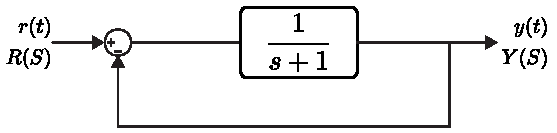
\includegraphics[width=0.4\textwidth]{ex1block}
    \end{center}
\end{minipage}
\end{center}

We already derived the Nyquist plot for this system

\begin{center}
\begin{minipage}[h]{\linewidth}
    \begin{center}
      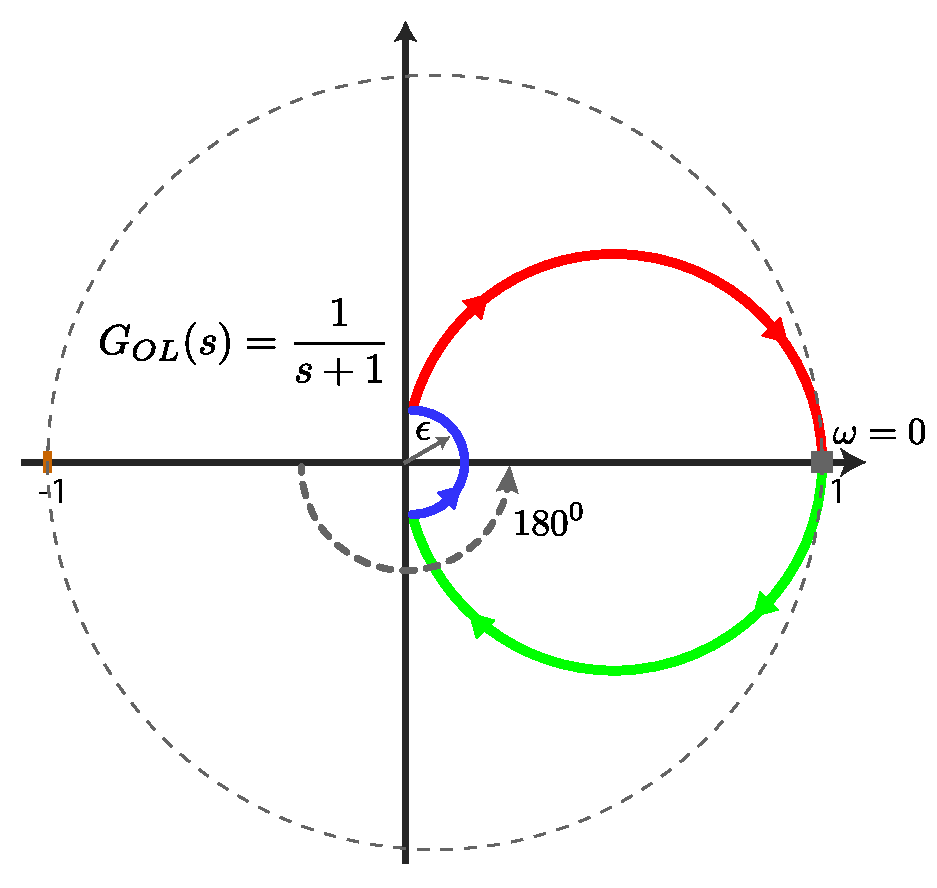
\includegraphics[width=0.4\textwidth]{ex1}
    \end{center}
\end{minipage}
\end{center}

We can see that the Real part of the polar polat is always 
positive, thus $g_m = \infty$. Where as the polar plot crosses
the unit circle only when $\omega = 0$, thus $\phi_m = 180^0$.

\newpage

\textbf{Ex:} Compute the gain margin and phase margin 
for the following closed-loop system for $K = 2$ and $K = 4$. 

\begin{center}
\begin{minipage}[h]{\linewidth}
    \begin{center}
      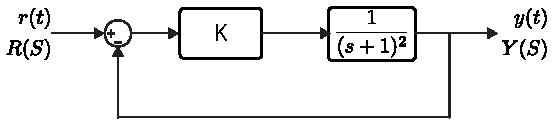
\includegraphics[width=0.4\textwidth]{ex2block}
    \end{center}
\end{minipage}
\end{center}

Nyquist plots for both gain cases is illustrated in the Figure below.
We can see from the illustration that 
%
\begin{align*}
  K &= 2 \Rightarrow \phi_m = 90^o \ \& \ g_m = \infty
  \\
  K &= 4 \Rightarrow \phi_m = 60^o \ \& \ g_m = \infty
\end{align*}

\begin{center}
\begin{minipage}[h]{\linewidth}
    \begin{center}
      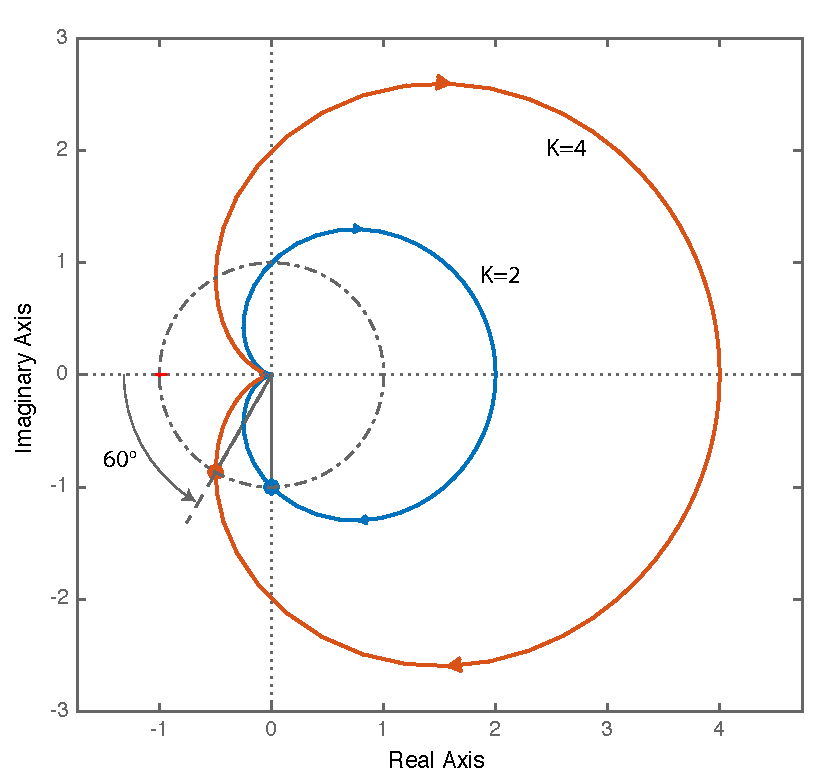
\includegraphics[width=0.75\textwidth]{ex2}
    \end{center}
\end{minipage}
\end{center}

Now let's try to compute the phase margins analytically.
Let's start with $K = 2$
%
\begin{align*}
  | G(j \omega_g) | &= 1 \ \rightarrow \  
                      \frac{2}{ \omega_g^2 + 1 }  = 1
  \rightarrow \ \omega_g = 1 
  \\
  \angle [ G(j) ] &= - 2 \angle [ j + 1 ] = -90^o 
  \\
 \phi_m &= 90^o  
\end{align*}
%
Now let's compute the phase margin for $K = 4$
%
\begin{align*}
  | G(j \omega_g) | &= 1 \ \rightarrow \  
                      \frac{4}{ \omega_g^2 + 1 }  = 1
  \rightarrow \ \omega_g = \sqrt{3}
  \\
  \angle [ G(j \sqrt{3}) ] &= - 2 \angle [ \sqrt{3} j + 1 ] = -120^o 
  \\
 \phi_m &= 60^o  
\end{align*}
%
Now let's compute the closed-loop transfer function
and compre the damping coefficients for both gain cases
%
\begin{align*}
  T_2 &= \frac{2}{s^2 + 2 s + 3} \ \rightarrow \ \zeta_2 = \frac{1}{\sqrt{3}}
        \\
  T_4 &= \frac{4}{s^2 + 2 s + 5} \ \rightarrow \ \zeta_2 = \frac{1}{\sqrt{5}}
\end{align*}
%
We can see that as we decrease the phase margin from $90^o$ to $60^o$,
we also decrease the damping ration which results in increased maximum-overshoot.
In general good phase margin provides good transent performance in time domain. 

\vspace{6pt}

\textbf{Ex:} Compute the gain margin and phase margin 
for the following closed-loop system for $K = 1$ and $K = 8$
and comment on the stability of the system for both cases. 

\begin{center}
\begin{minipage}[h]{\linewidth}
    \begin{center}
      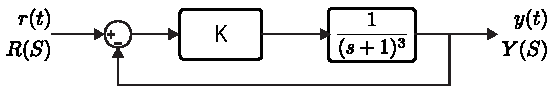
\includegraphics[width=0.4\textwidth]{ex3block}
    \end{center}
\end{minipage}
\end{center}

We already derived the Nyquist plot for the case $K = 1$,
now let's illustrate both Nyquist plots side-by-side.

\begin{center}
\begin{minipage}[h]{\linewidth}
    \begin{center}
      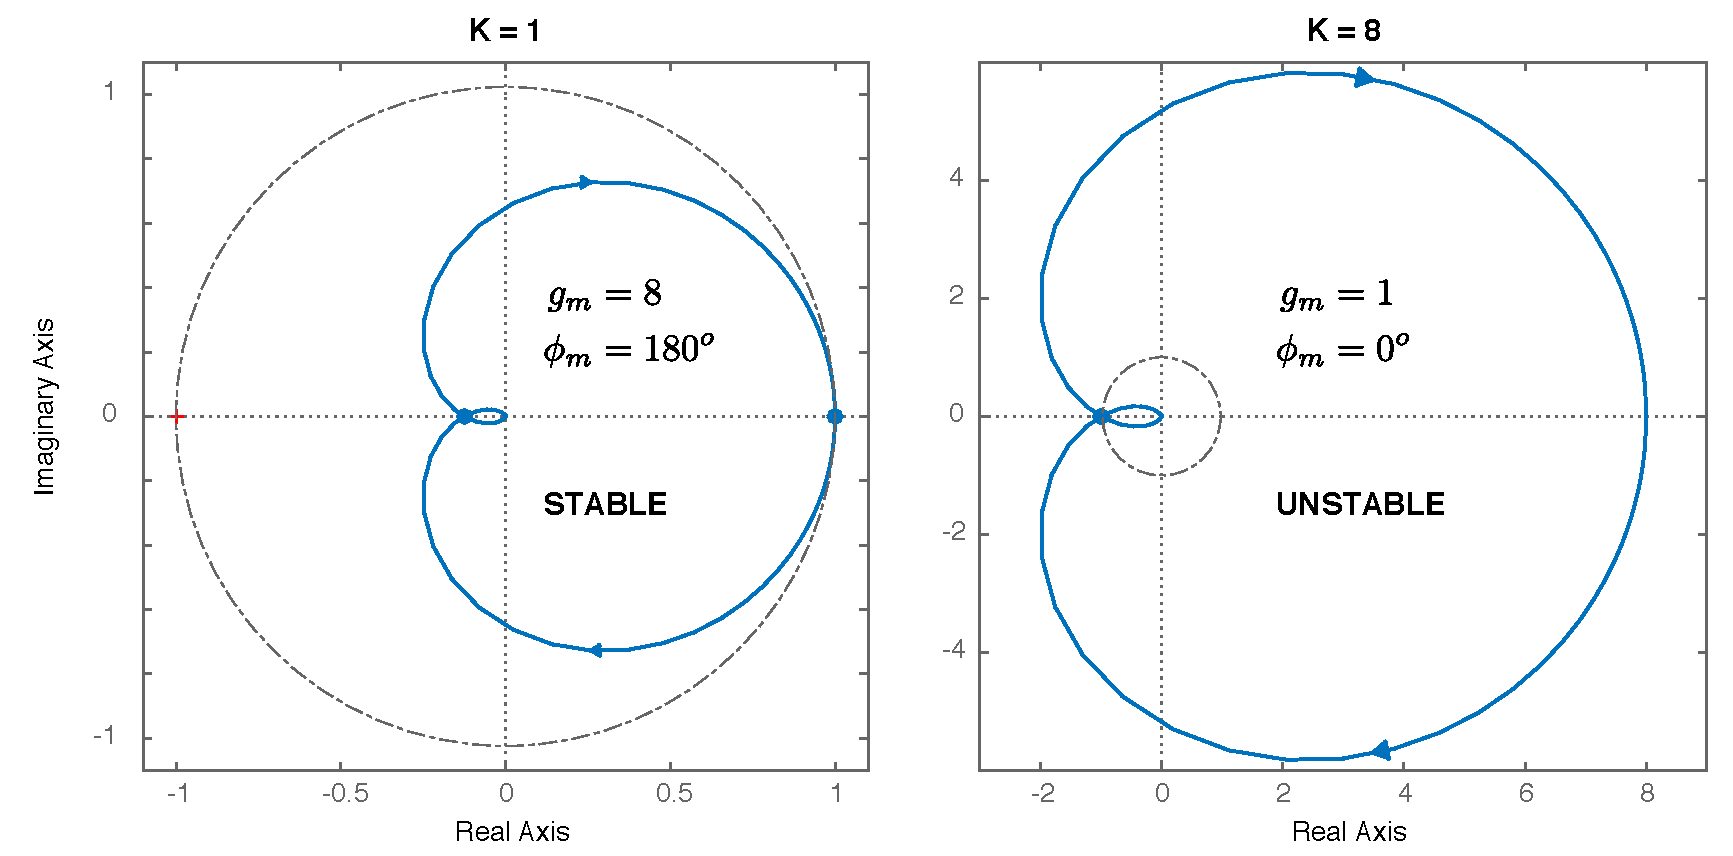
\includegraphics[width=0.99\textwidth]{ex3}
    \end{center}
\end{minipage}
\end{center}

\newpage

\textbf{Ex:} Compute the gain margin and phase margin 
for the following closed-loop system 

\begin{center}
\begin{minipage}[h]{\linewidth}
    \begin{center}
      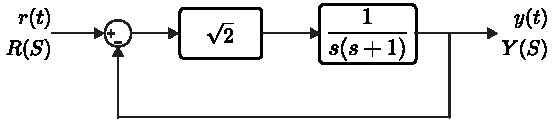
\includegraphics[width=0.4\textwidth]{ex4block}
    \end{center}
\end{minipage}
\end{center}

We already derived the Nyquist plot for the case $K = 1$,
now we have a different gain. Figure below illustrates 
the zoomed Nyquist plot (which is the important part
for gain and phase margin computations).

\vspace{6pt}

\begin{minipage}[h]{0.5\linewidth}
    \begin{center}
      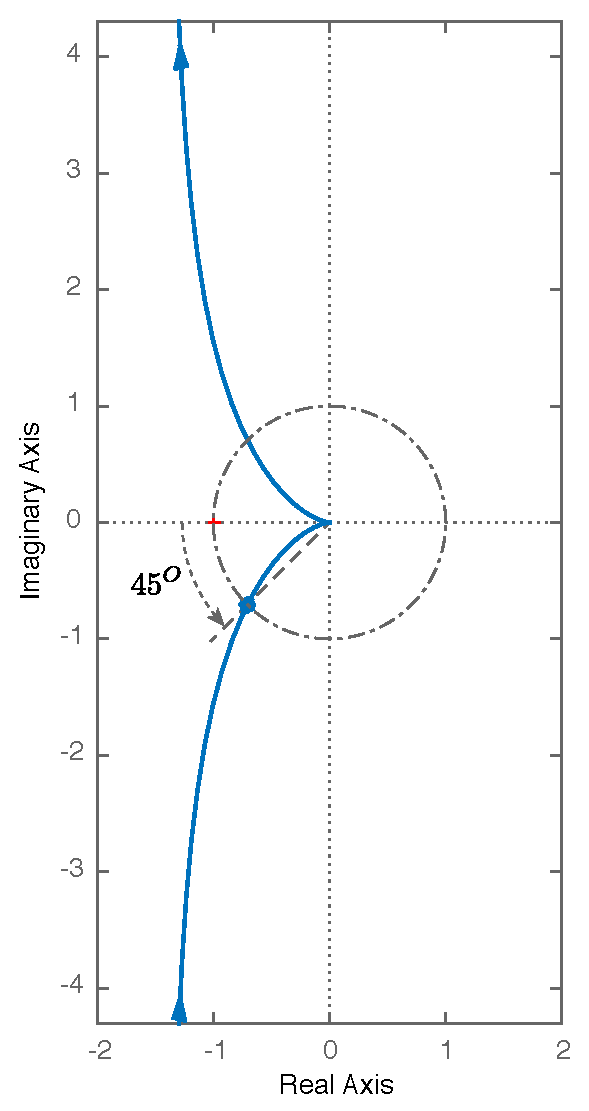
\includegraphics[width=0.99\textwidth]{ex4}
    \end{center}
\end{minipage}
\begin{minipage}[h]{0.5\linewidth}
    \begin{center}
      \begin{align*}
         & | G( j \omega_g ) | = 1 \ \rightarrow  | G( j \omega_g ) |^2 = 1
        \\
        & \frac{2}{\omega^2 (\omega^2 + 1)} = 1 
        \\
        & \rightarrow \ \omega_g = 1
          \\
        &\angle [ G( j ) ] = - ( 90^o+ 45^0) 
        \\
        &\phi_m = 45^0
        \\ 
        &g_m = \infty
      \end{align*}
    \end{center}
\end{minipage}


% **** This ENDS THE EXAMPLES. DON'T DELETE THE FOLLOWING LINE:
\end{document}